\chapter{An Investigation into the Security of RobotWeb}
The goal of this chapter is to understand how attackers will affect the functioning of the RobotWeb. First, we will posture about the aims of attackers, and how they would pursue them. Then we will dedicate the remainder of the chapter to answering the question of how successful they can be; first theoretically then empirically.

\section{The behaviour of an ideal attacker}
The RobotWeb allows robots to improve their localisations; these are likely to be used for navigational or control purposes. If a robot believes that it is too far left, its navigation/control system will instruct it to move right. This link between localisation and action is the prize sought after by attackers. If an attacker wishes for a robot to move right, it must simply convince it that it has moved too far left.

In addition to compromising others' localisations, an attacker will wish to keep its localisation uncompromised. This would mean that it would ignore any messages from robots that it has attacked, lest it inadvertently misinforms itself. However, this will come at a cost to the attacker, as it has fewer good sources of information about its localisation. If an attacker attacks all robots around it, it would effectively cut itself out of the RobotWeb, which leads us to believe that attackers would seek to perform targeted attacks. Here the attackers would either only attack a small number of robots, or attack robots at key times. Motivated attackers, seeking to attack all robots, may instead use a private version of the RobotWeb, where their attacks don't affect them.

Attackers will also wish to prevent their attacks from being easily identified, as those can be easily defended against. If their attacks are defended against, the overall effectiveness of an attacker is greatly diminished. Thus it stands to reason that attackers would aim to blend into the crowd, where their messages are indistinguishable from good messages. This means that an attacker is unlikely to try to convince robots that they are 100s of kilometers away, instead opting for more subtle differences.

Finally, when multiple attackers are present in an environment, it would be best for them to collaborate rather than compete. Competing attackers are likely to interfere with each others' attacks and thus reduce their overall efficacy. For this reason, we will ignore situations where this occurs.


\section{A simplified system}
Any theoretical investigation of the RobotWeb would require the investigator to analyse its backbone, the factor graph. However, the investigator would soon find themselves ensnared by complexity; caught in an intricate web of variable and factor nodes; messages constantly scurrying between them. Worse yet, the web would constantly be spun and unspun as robots moved closer and further from each other. In the face of this complexity, it becomes clear that simplification is needed.

To start, we choose to limit our investigation to a single variable, chosen arbitrarily, in the factor graph. Fortunately, the properties of Belief Propagation allow us to reason about this variable without loss of generality. Equation \ref{eqn:bp_belief} shows that the belief of a given variable is solely dependent on its connected factors. 

\begin{figure}[!h]
	\centering
	

\tikzset{every picture/.style={line width=0.75pt}} %set default line width to 0.75pt        

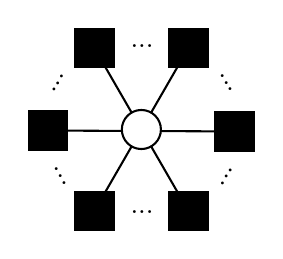
\begin{tikzpicture}[x=0.75pt,y=0.75pt,yscale=-1,xscale=1]
%uncomment if require: \path (0,288); %set diagram left start at 0, and has height of 288

%Shape: Square [id:dp5011100430912303] 
\draw  [fill={rgb, 255:red, 0; green, 0; blue, 0 }  ,fill opacity=1 ] (221.44,121.44) -- (240,121.44) -- (240,140) -- (221.44,140) -- cycle ;
%Shape: Square [id:dp1834276888413744] 
\draw  [fill={rgb, 255:red, 0; green, 0; blue, 0 }  ,fill opacity=1 ] (199.12,159.78) -- (217.68,159.78) -- (217.68,178.34) -- (199.12,178.34) -- cycle ;
%Shape: Square [id:dp4346063530366504] 
\draw  [fill={rgb, 255:red, 0; green, 0; blue, 0 }  ,fill opacity=1 ] (199.12,81.22) -- (217.68,81.22) -- (217.68,99.78) -- (199.12,99.78) -- cycle ;
%Straight Lines [id:da04926983509243965] 
\draw    (230.72,130.72) -- (140.72,130.28) ;
%Straight Lines [id:da6042872004378272] 
\draw    (208.4,169.06) -- (163.04,90.5) ;
%Straight Lines [id:da23454228445560488] 
\draw    (163.04,169.06) -- (208.4,90.5) ;
%Shape: Circle [id:dp7060474924289566] 
\draw  [fill={rgb, 255:red, 255; green, 255; blue, 255 }  ,fill opacity=1 ] (176.31,129.78) .. controls (176.31,124.59) and (180.53,120.37) .. (185.72,120.37) .. controls (190.91,120.37) and (195.13,124.59) .. (195.13,129.78) .. controls (195.13,134.97) and (190.91,139.19) .. (185.72,139.19) .. controls (180.53,139.19) and (176.31,134.97) .. (176.31,129.78) -- cycle ;
%Shape: Square [id:dp12209236616988428] 
\draw  [fill={rgb, 255:red, 0; green, 0; blue, 0 }  ,fill opacity=1 ] (131.44,121) -- (150,121) -- (150,139.56) -- (131.44,139.56) -- cycle ;
%Shape: Square [id:dp4564996494162272] 
\draw  [fill={rgb, 255:red, 0; green, 0; blue, 0 }  ,fill opacity=1 ] (153.76,159.78) -- (172.32,159.78) -- (172.32,178.34) -- (153.76,178.34) -- cycle ;
%Shape: Square [id:dp4857190958072921] 
\draw  [fill={rgb, 255:red, 0; green, 0; blue, 0 }  ,fill opacity=1 ] (153.76,81.22) -- (172.32,81.22) -- (172.32,99.78) -- (153.76,99.78) -- cycle ;

% Text Node
\draw (225,100) node [anchor=north west][inner sep=0.75pt]  [rotate=-60] [align=left] {...};
% Text Node
\draw (221.25,157.5) node [anchor=north west][inner sep=0.75pt]  [rotate=60] [align=left] {...};
% Text Node
\draw (179,87.5) node [anchor=north west][inner sep=0.75pt]   [align=left] {...};
% Text Node
\draw (145,145) node [anchor=north west][inner sep=0.75pt]  [rotate=-60] [align=left] {...};
% Text Node
\draw (179,167.5) node [anchor=north west][inner sep=0.75pt]   [align=left] {...};
% Text Node
\draw (140,112.5) node [anchor=north west][inner sep=0.75pt]  [rotate=60] [align=left] {...};


\end{tikzpicture}

	\caption[Single Variable in a Factor Graph]{A single variable connected to a number of factors}
\end{figure}

One problem still remains with the above setup - a single variable can be connected to any number of factors. As a further simplification, we can group the factors together based on their shared characteristics, which include their origin (if they are internal to the robot or not), their type (what kind of sensor they represent) and their intentions (whether they will help or hinder the robot). For our purposes, we will split the set of factors $F$, into distinct sets $G$ and $B$ based on whether the factors are ``good'' or ``bad'' for the robot. Good factors aim to steer the variable towards the ground truth value, while bad factors aim to steer it away. Notice that the sets $G$ and $B$ form a cover of $F$, that is $F = G \cup B$.

We then take this a step further and replace each set of factors with a single ``representative factor''.
\begin{figure}[!h]
	\centering
	

\tikzset{every picture/.style={line width=0.75pt}} %set default line width to 0.75pt        

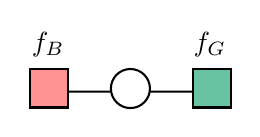
\begin{tikzpicture}[x=0.75pt,y=0.75pt,yscale=-1,xscale=1]
%uncomment if require: \path (0,171); %set diagram left start at 0, and has height of 171

%Straight Lines [id:da9426074160582016] 
\draw    (399.22,143.78) -- (359.94,143.66) ;
%Straight Lines [id:da643000004312603] 
\draw    (399.22,143.78) -- (438.5,143.66) ;
%Shape: Circle [id:dp3724334158586291] 
\draw  [fill={rgb, 255:red, 255; green, 255; blue, 255 }  ,fill opacity=1 ] (389.81,142.22) .. controls (389.81,137.03) and (394.02,132.81) .. (399.22,132.81) .. controls (404.41,132.81) and (408.62,137.03) .. (408.62,142.22) .. controls (408.62,147.41) and (404.41,151.63) .. (399.22,151.63) .. controls (394.02,151.63) and (389.81,147.41) .. (389.81,142.22) -- cycle ;
%Shape: Square [id:dp37804195853429245] 
\draw  [fill={rgb, 255:red, 255; green, 147; blue, 147 }  ,fill opacity=1 ] (350.66,132.81) -- (369.22,132.81) -- (369.22,151.37) -- (350.66,151.37) -- cycle ;
%Shape: Square [id:dp19659269496953535] 
\draw  [fill={rgb, 255:red, 104; green, 195; blue, 163 }  ,fill opacity=1 ] (429.22,132.81) -- (447.78,132.81) -- (447.78,151.37) -- (429.22,151.37) -- cycle ;

% Text Node
\draw (428.22,113.4) node [anchor=north west][inner sep=0.75pt]    {$f_{G}$};
% Text Node
\draw (350.22,113.4) node [anchor=north west][inner sep=0.75pt]    {$f_{B}$};


\end{tikzpicture}


	\caption[Representative factor graph around a single variable]{The above factor graph using ``representative factors''. $f_G$ and $f_B$ respectively represent the sets of good factors ($G$) and bad factors ($B$).}
\end{figure}

We calculate the messages from each of these representative factors as such:
\begin{eqnarray}
	m_{f_G \rightarrow x_i} = \underset{g \in G}{\prod} m_{f_g \rightarrow x_i}&
	m_{f_B \rightarrow x_i} = \underset{b \in B}{\prod} m_{f_b \rightarrow x_i}
\end{eqnarray}
Thus the belief of the variable becomes $p(x) = m_{f_G \rightarrow x} m_{f_B \rightarrow x}$, and since $G \cup B$ covers every factor connected to the variable, we can show that this replacement can be made without altering the variable's final result by equation \ref{eqn:bp_belief}.

\begin{equation}
	p(x_i) = \underset{s \in N(i)}{\prod} m_{f_s \rightarrow x_i}
	\tag{\ref{eqn:bp_belief}}
\end{equation}

For completeness, we now present the equations for contents of the messages $m_{f_G \rightarrow x_i}$ and $m_{f_B \rightarrow x_i}$. 
Each message has an information vector $\eta$ and a precision matrix $\Lambda$.
\begin{eqnarray}
	\eta_G = \underset{g \in G}{\sum} \eta_g&
	\Lambda_G = \underset{g \in G}{\sum} \Lambda_g \label{eqn:good_pull}\\
	\eta_B = \underset{b \in B}{\sum} \eta_b&
	\Lambda_B = \underset{b \in B}{\sum} \Lambda_b \label{eqn:bad_pull}
\end{eqnarray}

\section{Theoretical properties of the RobotWeb under attack}
\subsection{Measuring the strength of an attack}
From the above setup, we will now aim to quantify the strength of an attack. For mathematical convenience and ease of understanding, we will derive these equations in 1 dimension, and later present the n-dimensional forms.

To measure the strength of an attack we want to understand the impact of the bad factors on the variable's final belief. To do this we shall use the Kullback-Leibler (KL) divergence \citationneeded between the variable's belief when it is safe and when it is under attack.
The KL divergence is a measure of far the distribution Q is from the distribution P. The further the belief distribution under attack (BDA) is from the distribution suggested by the good factors, the stronger we say the attack is. Similarly, the closer the BDA is to the distribution suggested by the bad factors, the stronger the attack.

The KL divergence between 2 distributions of continuous random variables is:
\begin{equation}
	D_{KL}(P || Q) = \int_{-\infty}^{\infty} log\left( \frac{p(x)}{q(x)} \right) dx
\end{equation}

However a special case exists for Normal distributions, $N_1(\mu_1, \sigma_1^2)$ and $N_2(\mu_2, \sigma_2^2)$.
\begin{equation}
	D_{KL}(N_1 || N_2) = log\left(\frac{\sigma_2}{\sigma_1}\right) + \frac{\sigma_1^2 + (\mu_1 - \mu_2)^2}{2\sigma_2^2} - \frac{1}{2}
\end{equation}

In 1 dimension the messages sent from $f_G$ and $f_B$ are:
\begin{eqnarray}
	m_{f_G \rightarrow x_i} = (\eta_G, \Lambda_G) = (\frac{\mg}{\sgsq}, \frac{1}{\sgsq})\\
	m_{f_B \rightarrow x_i} = (\eta_B, \Lambda_B) = (\frac{\mb}{\sbsq}, \frac{1}{\sbsq}) \label{eqn:attacker_msg}
\end{eqnarray}

From \ref{eqn:bp_belief} we see that the BDA is equal to:
\begin{align}
	m_{f_G \rightarrow x} m_{f_B \rightarrow x} 
	&= (\eta_G + \eta_B, \Lambda_G + \Lambda_B)\\
	&= \left(\frac{\mg}{\sgsq} + \frac{\mb}{\sbsq}, \frac{1}{\sgsq} + \frac{1}{\sbsq}\right)\\
	&= \left(\frac{\mg\sbsq + \mb\sgsq}{\sgsq \sbsq}, \frac{\sbsq + \sgsq}{\sgsq \sbsq}\right)
\end{align}

The above distributions follow the following Normal distributions:
\begin{align}
	G &\sim N\left(\frac{\eta_G}{\Lambda_G}, \frac{1}{\Lambda_G}\right)\\
	B &\sim N\left(\frac{\eta_B}{\Lambda_B}, \frac{1}{\Lambda_B}\right)\\
	BDA &\sim N\left(\mu_{BDA}, \sigma_{BDA}^2\right)\\
	&\sim N\left(\frac{\eta_G + \eta_B}{\Lambda_G + \Lambda_B}, \frac{1}{\Lambda_G + \Lambda_B}\right)\\
	&\sim N\left(\frac{\mg\sbsq + \mb\sgsq}{\sgsq + \sbsq}, \frac{\sgsq \sbsq}{\sgsq + \sbsq}\right) \label{eqn:bda_distribution}
\end{align}

So now we take the KL divergence between the good factors' distribution $G$ and BDA. To make this easier to follow we derive each term in the sum separately.

First deriving the log term we get:
\begin{align}
	log\left(\frac{\sigma_{BDA}}{\sigma_{G}}\right)
	&= log\left(\sqrt[2]{\frac{\sigma_{BDA}^2}{\sigma_{G}^2}}\right)\\
	&= \frac{1}{2} log\left(\frac{\sigma_{BDA}^2}{\sigma_{G}^2}\right)\\
	&= \frac{1}{2} log\left(\frac{\sgsq \sbsq}{\sbsq + \sgsq} \times \frac{1}{\sgsq}\right)\\
	&= \frac{1}{2} log\left(\frac{\sbsq}{\sbsq + \sgsq}\right)
\end{align}

Next, we derive the fractional term:
\begin{align}
	\frac{\sigma_{G}^2 + (\mu_{G} - \mu_{BDA})^2}{2\sigma_{BDA}^2}
	&= \frac{
			\sgsq + \left(\mg - \frac{\mg\sbsq + \mb\sgsq}{\sbsq + \sgsq}\right)^2
		}{
			2 \frac{\sgsq \sbsq}{\sbsq + \sgsq}
		}\\
	&= \left(\sgsq + \left(\frac{\mg\sgsq + \mg\sbsq - \mg\sbsq - \mb\sgsq}{\sbsq + \sgsq}\right)^2\right) \times \frac{\sbsq + \sgsq}{2\sgsq\sbsq}\\
	&= \left(\sgsq + \left(\frac{\mg\sgsq - \mb\sgsq}{\sbsq + \sgsq}\right)^2\right) \times \frac{\sbsq + \sgsq}{2\sgsq\sbsq}\\
	&= \frac{\sgsq\left(\sgsq + \sbsq\right)^2 + \left(\mg\sgsq - \mb\sgsq\right)^2}{(\sbsq + \sgsq)^2} \times \frac{\sbsq + \sgsq}{2\sgsq\sbsq}\\
	&= \frac{\sgsq\left(\sgsq + \sbsq\right)^2 + \sigma_G^4\left(\mg - \mb\right)^2}{(\sbsq + \sgsq)^2} \times \frac{\sbsq + \sgsq}{2\sgsq\sbsq}\\
	&= \frac{\left(\sgsq + \sbsq\right)^2 + \sgsq\left(\mg - \mb\right)^2}{2\sbsq(\sbsq + \sgsq)}
\end{align}

Thus the KL divergence between $G$ and BDA is:
\begin{equation}
	\frac{1}{2} log\left(\frac{\sbsq}{\sbsq + \sgsq}\right) + \frac{\left(\sgsq + \sbsq\right)^2 + \sgsq\left(\mg - \mb\right)^2}{2\sbsq(\sbsq + \sgsq)} - \frac{1}{2}
\end{equation}

Similarly, the KL divergence between $B$ and BDA is:
\begin{equation}
	\frac{1}{2} log\left(\frac{\sgsq}{\sbsq + \sgsq}\right) + \frac{\left(\sgsq + \sbsq\right)^2 + \sbsq\left(\mg - \mb\right)^2}{2\sgsq(\sbsq + \sgsq)} - \frac{1}{2}
\end{equation}

From this, we notice a disturbing detail - the KL divergence is quadratically affected by the $\mb$. This suggests that the attacker's power is unbounded, so long as it chooses an appropriate $\sbsq$. This means that an attacker can suggest absurd localisations and have its victims believe them. For example, an attacker can convince its victims that they are on the opposite side of the planet!

\subsection{Crafting the perfect message}
From the results derived in the previous section, we know that, theoretically, an attacker will seek to increase its $\mb$ to $\infty$ and decrease its $\sbsq$ to 0. However, in a real-life scenario, it is unlikely that the attacker would fully exploit these powers, for two reasons.
\begin{enumerate}
	\item Robots are unlikely to believe \textit{incredibly} incorrect values - no sensible robot would believe that it has moved 500km away in the past 3 seconds.
	\item Robots don't have infinite numerical precision, so large values of $\Lambda_B$ ($\frac{1}{\sbsq}$) would cause overflow errors, which would prevent the attacker from controlling the robot's belief.
\end{enumerate}

Given these restrictions, attackers would set their values of $\mb$ to believable values, whilst choosing the largest value of $\sbsq$ possible. 
We will now suppose that the attacker wishes to move its victim's belief from $\mg$ to $\mt$.
As before, the attacker sends a message with the form described in equation \ref{eqn:attacker_msg}.

So from equation \ref{eqn:bda_distribution}, we see that:
\begin{equation}
	\mt = \frac{\mg\sbsq + \mb\sgsq}{\sgsq + \sbsq}
\end{equation}

Which can be rearranged into the form:
\begin{equation}
	\mb = \frac{\mt\left(\sgsq + \sbsq\right) - \mg\sbsq}{\sgsq}
\end{equation}

Which can be used to calculate the $\mb$ that an attacker would send given a minimum $\sbsq$. 
Thus the attacker would send the following message:
\begin{equation}
	\left(\frac{\mt\left(\sgsq + \sbsq\right) - \mg\sbsq}{\sgsq\sbsq}, \frac{1}{\sbsq}\right)
\end{equation}

\subsection{Scaling back up to n-dimensional space}
For completeness, we now present the KL divergence between the BDA and G distributions in k-dimensions.

The KL divergence between 2 k-variate Normal distributions, $N_1(\boldsymbol{\mu_1}, \Sigma_1)$ and $N_2(\boldsymbol{\mu_2}, \Sigma_2)$ is:
\begin{equation}
	KL\left[P || Q \right] = \frac{1}{2}\left[
		tr(\Sigma_2^{-1}\Sigma_1) + \left(\boldsymbol{\mu_2} - \boldsymbol{\mu_1}\right)^T \Sigma_2^{-1} \left(\boldsymbol{\mu_2} - \boldsymbol{\mu_1}\right) - k + log\left(\frac{det \; \Sigma_2}{det \; \Sigma_1}\right)
	\right]
\end{equation}

Using this with the messages sent from $f_G$ and $f_B$, we find that the KL divergence between G and BDA is:

\begin{gather}
	\frac{1}{2} \left[
		tr\left(\Lambda_B\Lambda_G^{-1}\right) +
		\left(\boldsymbol{\mu_{BDA}} - \boldsymbol{\mu_G}\right)^T \left(\Lambda_G + \Lambda_B\right) \left(\boldsymbol{\mu_{BDA}} - \boldsymbol{\mu_G}\right) + log\left(\frac{det \; \Lambda_G}{det \; \left(\Lambda_G + \Lambda_B\right)}\right)
	\right]\\
	\text{where}\nonumber\\
	\boldsymbol{\mu_{BDA}} = \left(\Lambda_G + \Lambda_B\right) \left(\eta_G + \eta_B\right)\nonumber
\end{gather}

\subsection{The Force-Based model of attacks}
From the above analysis, we believe that attacks can be reasoned about using a ``Force-Based Model''. Here we think of all messages sent to a variable as forces pulling the variable to particular localisations. Every good message will pull the variable towards the ground truth value, whilst every bad message will pull it towards an alternative localisation. The strength of a message's ``pull'' corresponds to the eigenvalues of its $\Lambda$ matrix, where the higher the eigenvalues, the stronger the pull is.

If two messages pull the robot towards the same localisation, then their forces will be additively combined, increasing their overall strength. However, if the messages pull the robot to diametrically opposed localisations, then their forces will cancel out. Once all forces have been resolved, the variable will move to the localisation suggested by the resultant force. The strength of the variable's conviction is determined by the strength of this resultant force.

\section{Hypotheses}
Now using the ``Force-Based Model'', we form 6 hypotheses about the behaviour of the entire RobotWeb under attack. Later, we will experimentally verify each of these hypotheses.

\subsection{There is Strength in Numbers} \label{hyp:strength_in_numbers}
As the number of good robots rises, the effectiveness of an attack will fall. We believe that this can be seen through the lens of the ``Force-Based Model'' where, as the number of good robots increases, so does the overall number of good messages, which in turn increases the overall force pulling the robots towards the truth. This will increase the resistance against any given attack, decreasing the strength of the resultant force.

However, it is unlikely that a large number of good robots will be able to nullify attacks, as the attacker will likely respond by increasing the strength of its messages. Since the good robots cannot freely increase $\Lambda$, they will once again conform to the attacker's wishes.

\subsection{Long Memories are Detrimental} \label{hyp:history} % History can be weaponised
One little discussed feature of the RobotWeb so far has been its time-windowed history. Instead of remembering every past position that that robot has had, it instead chooses to only remember the past $h$ positions. This improves the performance of robots in the RobotWeb, as they store fewer pose variables and thus perform fewer floating-point operations when updating beliefs. In the original paper, Murai et al. show that the impact of time-windowed history on the average performance of each robot is negligible.

%TODO: get original

\begin{figure}[!h]
    \centering
    \makebox[\textwidth]{\includegraphics[width=\textwidth]{diagrams/history.png}}
	\caption[The negligible effect of using time-windowed history]{Graphs showing a negligible decrease in performance between using a full history vector and only using the previous 5 pose variables. Taken from \cite[Figure~3]{Robotweb}}
\end{figure}


However, we believe that keeping the full position history not only harms the computational performance of a robot but also amplifies the strength of attacks. If an attacker can successfully attack a robot at time $t$, then the pose variable at $t$, $v_t$ will contain a $\mu$ close to the attacker's target $\mu$, and its $\Lambda$ will be high. Then in the next step, this corrupted $v_t$ will pull the robot towards the attacker's target instead of towards a ground truth. As the size of this history increases, so does the total pull it will have on the robot.

Note: During the early stages of an attack, we believe that longer histories will serve as a small counterbalance to the attacker, but as their strength is limited, they will be unable to significantly prevent an attack. Thus we believe that they are more harmful than helpful.

\subsection{Attacks are Contagious} \label{hyp:contagion} % A falling tide sinks all ships/Can't let the genie out of the bottle
Similarly to the previous hypothesis, we can assume that any other variable connected to $v_t$ will be attacked by it. Thus a victim of an attack will unintentionally attack all those it contacts, leading us to hypothesise that attacks have a degree of contagion. 

Attackers may not be able to prevent or limit contagion, as they would need to strongly pull unintentional victims back to a ground truth value. Since no robot has absolute certainty about the locations of any other, the attacker will pull them to values close to their ground truth. Yet, as there is no mechanism to decrease $\Lambda$, the attacker will still make the other robots overconfident about their locations, which may bias them in the long term.

\subsection{Young Robots are the most Vulnerable} \label{hyp:startup_vuln}
Robots which are have only recently joined the RobotWeb (and hence can be considered ``young'') are unlikely to have strong beliefs about their localisation. As they participate in the RobotWeb, the strength of their beliefs will increases. However, these initial weak beliefs will translate to a weaker pull towards the ground truth, and provide a weaker resistance to attackers.

We believe that this effect may be strongly linked to the robot's history size, as once the history size has been exhausted, the robot will only make marginal gains from experience.

\subsection{Bounds on $\mu$ can be slowly escaped} \label{hyp:mu_bound}
An intuitive defence against the attackers is setting an upper bound on how far a message can suggest the robot is from its current position belief. 
However, we believe that this approach is ineffective, and can be easily evaded by attackers. In this subsection, we will lay out how this defence would work and how it can be bypassed.

For the upper bound to be effective, it must occupy a ``Goldilocks zone'' - it cannot be too large or too small. If the upper bound is too large, it would present attackers with ample opportunities to control the robot's belief, especially since they aim to suggest somewhat plausible positions.
If the upper bound is too small, it would effectively prevent the robot from listening to any dissenting messages from other good robots.

Now suppose that at time $t$, the robot is at position $\mu_t$ and has an upper bound of $\epsilon$. It would then evaluate each incoming message and reject it if its proposed position $\mu'_t$ is a distance $\epsilon$ away from $\mu_t$. After filtering out all ``bad'' messages, the robot would use the remaining messages to determine $\mu_{t+1}$. 

Being aware of this scheme, an attacker would seek to incrementally attack the robot. It would start by proposing a position $\mu''_t$ that lies between $\mu_t$ and its target location $\mu'_t$, such that $\mu''_t$ is accepted by the robot. This would successfully shift the robot's position estimate $\mu_{t+1}$ to $\mu''_t$. In the next iteration, the robot would reject any proposals a distance of $\epsilon$ away from $\mu_{t+1} = \mu''_t$. Hence over several iterations, the robot's position estimate would slowly shift to $\mu'_t$, and thus the attacker would be able to escape the bound.
% \todo{Would a diagram be useful here?}

\subsection{Bounds on $\Lambda$ can be quickly escaped} \label{hyp:sybils}
As shown previously, the strength of an attack is highly dependent on its ability to propose arbitrary values of $\Lambda$. This leads to another intuitive defence strategy - robots set an upper bound on the $\Lambda$ values that they receive. We believe that this strategy is effective when there is only a single identity spreading misinformation, counterbalanced by many others sending reliable information. In this subsection, we will provide a justification for this belief as well as a strategy that an attacker could take to bypass the upper bound on $\Lambda$.

When sending a message, each robot decides the strength of the message's pull. Good robots limit their strength to the accuracy of their sensors, while attackers will set their strength to the fullest extent. This once again makes the case for the use of a reasonable upper bound on the strength of a message, similar to the one described above.

However, we argue that this upper bound is unenforceable in practice, for an attacker can simply ``split'' their message into several weaker parts. So far in our analysis, we have treated $\Lambda_B$ as if it were sent in a single message, however from equation \ref{eqn:bad_pull} we can see that it may also be the result of several bad robots sending messages. If the upper bound on an individual message's $\Lambda$ is $\lambda$, then an attacker could simply send several messages from several different identities to arrive at a strong $\Lambda_B$, in a Sybil Attack. Here the strengths of each Sybil's message will increase the overall strength of the attacking force, while each message's $\Lambda$ will fly under the bound.


\subsubsection{Aside: Attacks are uncorrelated} \label{hyp:uncorrelated_sybils}
Considering the ``Force-Based Model'' of variables, it stands to reason that in a Sybil Attack, the messages sent by individual identities will not be correlated with each other, as that would greatly simplify the detection and prevention of attacks. Instead, we believe that Sybil Attackers would send messages with wildly different $\mu$ values, that would resolve to the actual attack that the attacker intends.

Consequently, it becomes impossible to detect whether a message belongs to an attacker based on its contents.

\section{Experimental evidence}

Now, we will evaluate the above hypotheses in a simulated environment. Our goal is to show that the predicted phenomena can arise, rather than guaranteeing their emergence. The reasoning behind this is that an attack only needs to be successful in a single situation for it to be considered potent.

\subsection{Experimental setup}
We will use an adapted version of the simulator detailed in \cite[RobotWeb]{Robotweb} for our experiments. Each simulation will contain a single attacking robot and $n$ normal robots. Each robot will move along a predefined path, and aim to localise well to that path - this will be challenged by the attacker, which will attempt to trick them into localising to a path of its choosing.

Furthermore, each robot in the simulation will carry 2 sensors; one for odometry and one for measuring others. The odometry sensor will be used by a robot to estimate its current location using its previous location and its motion. The range-bearing sensor will be used to measure other robots - it will measure the distance between the 2 robots and the bearing of the other robot from this one. All robots' range-bearing sensors have a range limit; however, attackers will ignore this as they always know where they want their victims to be.

The simulation has several configurable parameters which we will vary in our experiments. We detail the most important ones below.

% TODO: make table good
% QUESTION: Should I explain how likely robots are to measure each other?
% TODO: Include startup delay
\renewcommand{\arraystretch}{1.35}
\begin{table}[ht!]
\centering
\begin{tabular}{|c|c|c|}
\hline
\textbf{Parameter}    & \textbf{Description}                                                                                                          & \textbf{Default values}                                                                                        \\ \hline
Dataset               & The physical path travelled by each robot.                                                                                    & See below                                                                                                      \\ \hline
Attacker Dataset      & \begin{tabular}[c]{@{}c@{}}The path attackers attempt to trick the robot \\ into localising onto\end{tabular}                 & See below                                                                                                      \\ \hline
History size & \begin{tabular}[c]{@{}c@{}}The number of past pose variables \\ used by each robot.\end{tabular} & 1                                                                                                             \\ \hline
N iterations per step & \begin{tabular}[c]{@{}c@{}}The number of GBP iterations performed\\  every time the robot moves.\end{tabular}                 & 10                                                                                                             \\ \hline
SE2 Prior             & The accuracy of each robot's original position.                                                                               & \begin{tabular}[c]{@{}c@{}}$\sigma_x = 1e^{-8}$ m\\ $\sigma_y = 1e^{-8}$ m\end{tabular}                        \\ \hline
Between SE2           & The accuracy of each robot's odometry sensor.                                                                                 & \begin{tabular}[c]{@{}c@{}}$\sigma_x = 0.1$ m\\  $\sigma_y = 0.1$ m \\ $\sigma_\theta = 0.01$ rad\end{tabular} \\ \hline
Sensor range limit    & The furthest a range-bearing sensor can detect.                                                                               & 0.25 m                                                                                                         \\ \hline
Sensor noise model    & \begin{tabular}[c]{@{}c@{}}The noise associated with the \\ range and bearing measurements.\end{tabular}                      & \begin{tabular}[c]{@{}c@{}}$\sigma_r = 0.05$ m\\ $\sigma_\theta = 0.1$ rad\end{tabular}                        \\ \hline
Attacker confidence   & \begin{tabular}[c]{@{}c@{}}The confidence claimed by the attacker.\end{tabular}                      & \begin{tabular}[c]{@{}c@{}}$\sigma_x = 0.001$ m\\ $\sigma_y = 0.001$ m\end{tabular} \\ \hline
\end{tabular}
\end{table}

\subsubsection{Path design}
Since the RobotWeb currently hasn't been deployed, we are faced with a dearth of real-world paths for our experiments. This leaves us with the choice of either inventing a realistic path or using a simple, artificial path. For the following experiments, we have chosen to use simple paths as we aim to show that these phenomena can arise. Later we will test our defences on more realistic paths.

\begin{figure}[!h]
	\centering
	

\tikzset{every picture/.style={line width=0.75pt}} %set default line width to 0.75pt        

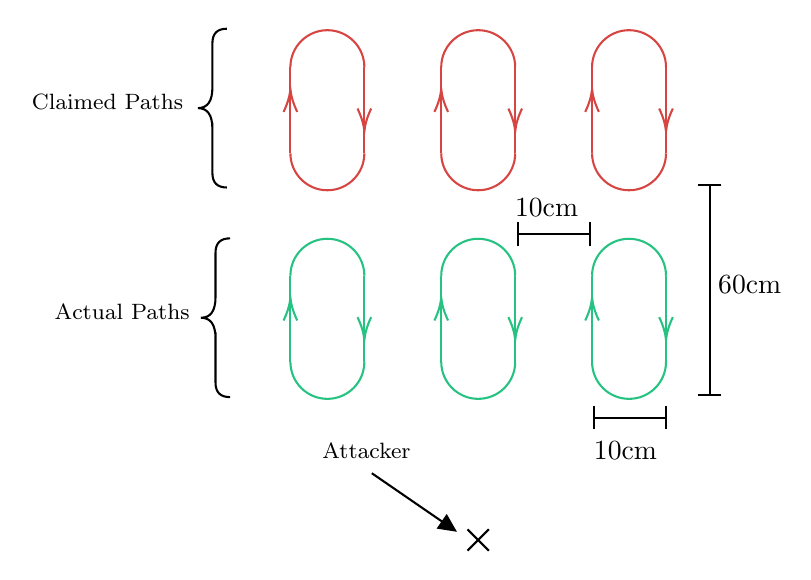
\begin{tikzpicture}[x=0.75pt,y=0.75pt,yscale=-1,xscale=1]
%uncomment if require: \path (0,300); %set diagram left start at 0, and has height of 300

%Shape: Arc [id:dp0857149156348076] 
\draw  [draw opacity=0] (129.08,53.57) .. controls (129.08,53.57) and (129.08,53.57) .. (129.08,53.57) .. controls (129.08,43.74) and (137.06,35.76) .. (146.9,35.76) .. controls (156.74,35.76) and (164.71,43.74) .. (164.71,53.57) -- (146.9,53.57) -- cycle ; \draw  [color={rgb, 255:red, 214; green, 69; blue, 65 }  ,draw opacity=1 ] (129.08,53.57) .. controls (129.08,53.57) and (129.08,53.57) .. (129.08,53.57) .. controls (129.08,43.74) and (137.06,35.76) .. (146.9,35.76) .. controls (156.74,35.76) and (164.71,43.74) .. (164.71,53.57) ;  
%Straight Lines [id:da5322421522198548] 
\draw [color={rgb, 255:red, 214; green, 69; blue, 65 }  ,draw opacity=1 ]   (129.08,53.57) -- (129.08,95.07) ;
%Shape: Arc [id:dp2308989347294783] 
\draw  [draw opacity=0] (164.71,95.07) .. controls (164.71,95.07) and (164.71,95.07) .. (164.71,95.07) .. controls (164.71,104.91) and (156.74,112.88) .. (146.9,112.88) .. controls (137.06,112.88) and (129.08,104.91) .. (129.08,95.07) -- (146.9,95.07) -- cycle ; \draw  [color={rgb, 255:red, 214; green, 69; blue, 65 }  ,draw opacity=1 ] (164.71,95.07) .. controls (164.71,95.07) and (164.71,95.07) .. (164.71,95.07) .. controls (164.71,104.91) and (156.74,112.88) .. (146.9,112.88) .. controls (137.06,112.88) and (129.08,104.91) .. (129.08,95.07) ;  
%Straight Lines [id:da5629844829721629] 
\draw [color={rgb, 255:red, 214; green, 69; blue, 65 }  ,draw opacity=1 ]   (164.71,53.57) -- (164.71,95.07) ;

%Straight Lines [id:da6879257912498304] 
\draw [color={rgb, 255:red, 214; green, 69; blue, 65 }  ,draw opacity=1 ]   (129.08,84.45) -- (129.08,66.19) ;
\draw [shift={(129.08,64.19)}, rotate = 90] [color={rgb, 255:red, 214; green, 69; blue, 65 }  ,draw opacity=1 ][line width=0.75]    (10.93,-3.29) .. controls (6.95,-1.4) and (3.31,-0.3) .. (0,0) .. controls (3.31,0.3) and (6.95,1.4) .. (10.93,3.29)   ;
%Straight Lines [id:da78952208923761] 
\draw [color={rgb, 255:red, 214; green, 69; blue, 65 }  ,draw opacity=1 ]   (164.71,82.45) -- (164.71,64.19) ;
\draw [shift={(164.71,84.45)}, rotate = 270] [color={rgb, 255:red, 214; green, 69; blue, 65 }  ,draw opacity=1 ][line width=0.75]    (10.93,-3.29) .. controls (6.95,-1.4) and (3.31,-0.3) .. (0,0) .. controls (3.31,0.3) and (6.95,1.4) .. (10.93,3.29)   ;

%Shape: Arc [id:dp943258450102171] 
\draw  [draw opacity=0] (201.75,53.57) .. controls (201.75,43.74) and (209.73,35.76) .. (219.57,35.76) .. controls (229.41,35.76) and (237.39,43.74) .. (237.39,53.57) -- (219.57,53.57) -- cycle ; \draw  [color={rgb, 255:red, 214; green, 69; blue, 65 }  ,draw opacity=1 ] (201.75,53.57) .. controls (201.75,43.74) and (209.73,35.76) .. (219.57,35.76) .. controls (229.41,35.76) and (237.39,43.74) .. (237.39,53.57) ;  
%Straight Lines [id:da7460858686327427] 
\draw [color={rgb, 255:red, 214; green, 69; blue, 65 }  ,draw opacity=1 ]   (201.75,53.57) -- (201.75,95.07) ;
%Shape: Arc [id:dp7505919410049695] 
\draw  [draw opacity=0] (237.39,95.07) .. controls (237.39,104.91) and (229.41,112.88) .. (219.57,112.88) .. controls (209.73,112.88) and (201.75,104.91) .. (201.75,95.07) -- (219.57,95.07) -- cycle ; \draw  [color={rgb, 255:red, 214; green, 69; blue, 65 }  ,draw opacity=1 ] (237.39,95.07) .. controls (237.39,104.91) and (229.41,112.88) .. (219.57,112.88) .. controls (209.73,112.88) and (201.75,104.91) .. (201.75,95.07) ;  
%Straight Lines [id:da5413783734225774] 
\draw [color={rgb, 255:red, 214; green, 69; blue, 65 }  ,draw opacity=1 ]   (237.39,53.57) -- (237.39,95.07) ;

%Straight Lines [id:da6345338713179298] 
\draw [color={rgb, 255:red, 214; green, 69; blue, 65 }  ,draw opacity=1 ]   (201.75,84.45) -- (201.75,66.19) ;
\draw [shift={(201.75,64.19)}, rotate = 90] [color={rgb, 255:red, 214; green, 69; blue, 65 }  ,draw opacity=1 ][line width=0.75]    (10.93,-3.29) .. controls (6.95,-1.4) and (3.31,-0.3) .. (0,0) .. controls (3.31,0.3) and (6.95,1.4) .. (10.93,3.29)   ;
%Straight Lines [id:da7349959112756272] 
\draw [color={rgb, 255:red, 214; green, 69; blue, 65 }  ,draw opacity=1 ]   (237.39,82.45) -- (237.39,64.19) ;
\draw [shift={(237.39,84.45)}, rotate = 270] [color={rgb, 255:red, 214; green, 69; blue, 65 }  ,draw opacity=1 ][line width=0.75]    (10.93,-3.29) .. controls (6.95,-1.4) and (3.31,-0.3) .. (0,0) .. controls (3.31,0.3) and (6.95,1.4) .. (10.93,3.29)   ;

%Shape: Arc [id:dp4454600887945992] 
\draw  [draw opacity=0] (274.42,53.57) .. controls (274.42,43.74) and (282.39,35.76) .. (292.23,35.76) .. controls (302.07,35.76) and (310.05,43.74) .. (310.05,53.57) -- (292.23,53.57) -- cycle ; \draw  [color={rgb, 255:red, 214; green, 69; blue, 65 }  ,draw opacity=1 ] (274.42,53.57) .. controls (274.42,43.74) and (282.39,35.76) .. (292.23,35.76) .. controls (302.07,35.76) and (310.05,43.74) .. (310.05,53.57) ;  
%Straight Lines [id:da3535450240320428] 
\draw [color={rgb, 255:red, 214; green, 69; blue, 65 }  ,draw opacity=1 ]   (274.42,53.57) -- (274.42,95.07) ;
%Shape: Arc [id:dp07519283691274281] 
\draw  [draw opacity=0] (310.05,95.07) .. controls (310.05,104.91) and (302.07,112.88) .. (292.23,112.88) .. controls (282.39,112.88) and (274.42,104.91) .. (274.42,95.07) -- (292.23,95.07) -- cycle ; \draw  [color={rgb, 255:red, 214; green, 69; blue, 65 }  ,draw opacity=1 ] (310.05,95.07) .. controls (310.05,104.91) and (302.07,112.88) .. (292.23,112.88) .. controls (282.39,112.88) and (274.42,104.91) .. (274.42,95.07) ;  
%Straight Lines [id:da4596754592263743] 
\draw [color={rgb, 255:red, 214; green, 69; blue, 65 }  ,draw opacity=1 ]   (310.05,53.57) -- (310.05,95.07) ;

%Straight Lines [id:da4148525058433936] 
\draw [color={rgb, 255:red, 214; green, 69; blue, 65 }  ,draw opacity=1 ]   (274.42,84.45) -- (274.42,66.19) ;
\draw [shift={(274.42,64.19)}, rotate = 90] [color={rgb, 255:red, 214; green, 69; blue, 65 }  ,draw opacity=1 ][line width=0.75]    (10.93,-3.29) .. controls (6.95,-1.4) and (3.31,-0.3) .. (0,0) .. controls (3.31,0.3) and (6.95,1.4) .. (10.93,3.29)   ;
%Straight Lines [id:da40569561359945716] 
\draw [color={rgb, 255:red, 214; green, 69; blue, 65 }  ,draw opacity=1 ]   (310.05,82.45) -- (310.05,64.19) ;
\draw [shift={(310.05,84.45)}, rotate = 270] [color={rgb, 255:red, 214; green, 69; blue, 65 }  ,draw opacity=1 ][line width=0.75]    (10.93,-3.29) .. controls (6.95,-1.4) and (3.31,-0.3) .. (0,0) .. controls (3.31,0.3) and (6.95,1.4) .. (10.93,3.29)   ;


%Shape: Arc [id:dp9600264214104561] 
\draw  [draw opacity=0] (129.08,154.07) .. controls (129.08,154.07) and (129.08,154.07) .. (129.08,154.07) .. controls (129.08,144.24) and (137.06,136.26) .. (146.9,136.26) .. controls (156.74,136.26) and (164.71,144.24) .. (164.71,154.07) -- (146.9,154.07) -- cycle ; \draw  [color={rgb, 255:red, 38; green, 194; blue, 129 }  ,draw opacity=1 ] (129.08,154.07) .. controls (129.08,154.07) and (129.08,154.07) .. (129.08,154.07) .. controls (129.08,144.24) and (137.06,136.26) .. (146.9,136.26) .. controls (156.74,136.26) and (164.71,144.24) .. (164.71,154.07) ;  
%Straight Lines [id:da06283910895753198] 
\draw [color={rgb, 255:red, 38; green, 194; blue, 129 }  ,draw opacity=1 ]   (129.08,154.07) -- (129.08,195.57) ;
%Shape: Arc [id:dp8022390792858354] 
\draw  [draw opacity=0] (164.71,195.57) .. controls (164.71,195.57) and (164.71,195.57) .. (164.71,195.57) .. controls (164.71,205.41) and (156.74,213.38) .. (146.9,213.38) .. controls (137.06,213.38) and (129.08,205.41) .. (129.08,195.57) -- (146.9,195.57) -- cycle ; \draw  [color={rgb, 255:red, 38; green, 194; blue, 129 }  ,draw opacity=1 ] (164.71,195.57) .. controls (164.71,195.57) and (164.71,195.57) .. (164.71,195.57) .. controls (164.71,205.41) and (156.74,213.38) .. (146.9,213.38) .. controls (137.06,213.38) and (129.08,205.41) .. (129.08,195.57) ;  
%Straight Lines [id:da5702202677205794] 
\draw [color={rgb, 255:red, 38; green, 194; blue, 129 }  ,draw opacity=1 ]   (164.71,154.07) -- (164.71,195.57) ;

%Straight Lines [id:da5596372875774243] 
\draw [color={rgb, 255:red, 38; green, 194; blue, 129 }  ,draw opacity=1 ]   (129.08,184.95) -- (129.08,166.69) ;
\draw [shift={(129.08,164.69)}, rotate = 90] [color={rgb, 255:red, 38; green, 194; blue, 129 }  ,draw opacity=1 ][line width=0.75]    (10.93,-3.29) .. controls (6.95,-1.4) and (3.31,-0.3) .. (0,0) .. controls (3.31,0.3) and (6.95,1.4) .. (10.93,3.29)   ;
%Straight Lines [id:da4662112490696484] 
\draw [color={rgb, 255:red, 38; green, 194; blue, 129 }  ,draw opacity=1 ]   (164.71,182.95) -- (164.71,164.69) ;
\draw [shift={(164.71,184.95)}, rotate = 270] [color={rgb, 255:red, 38; green, 194; blue, 129 }  ,draw opacity=1 ][line width=0.75]    (10.93,-3.29) .. controls (6.95,-1.4) and (3.31,-0.3) .. (0,0) .. controls (3.31,0.3) and (6.95,1.4) .. (10.93,3.29)   ;

%Shape: Arc [id:dp4562159985401648] 
\draw  [draw opacity=0] (201.75,154.07) .. controls (201.75,144.24) and (209.73,136.26) .. (219.57,136.26) .. controls (229.41,136.26) and (237.39,144.24) .. (237.39,154.07) -- (219.57,154.07) -- cycle ; \draw  [color={rgb, 255:red, 38; green, 194; blue, 129 }  ,draw opacity=1 ] (201.75,154.07) .. controls (201.75,144.24) and (209.73,136.26) .. (219.57,136.26) .. controls (229.41,136.26) and (237.39,144.24) .. (237.39,154.07) ;  
%Straight Lines [id:da19157667291963465] 
\draw [color={rgb, 255:red, 38; green, 194; blue, 129 }  ,draw opacity=1 ]   (201.75,154.07) -- (201.75,195.57) ;
%Shape: Arc [id:dp13013570223308513] 
\draw  [draw opacity=0] (237.39,195.57) .. controls (237.39,205.41) and (229.41,213.38) .. (219.57,213.38) .. controls (209.73,213.38) and (201.75,205.41) .. (201.75,195.57) -- (219.57,195.57) -- cycle ; \draw  [color={rgb, 255:red, 38; green, 194; blue, 129 }  ,draw opacity=1 ] (237.39,195.57) .. controls (237.39,205.41) and (229.41,213.38) .. (219.57,213.38) .. controls (209.73,213.38) and (201.75,205.41) .. (201.75,195.57) ;  
%Straight Lines [id:da19897438711687387] 
\draw [color={rgb, 255:red, 38; green, 194; blue, 129 }  ,draw opacity=1 ]   (237.39,154.07) -- (237.39,195.57) ;

%Straight Lines [id:da9802863492139731] 
\draw [color={rgb, 255:red, 38; green, 194; blue, 129 }  ,draw opacity=1 ]   (201.75,184.95) -- (201.75,166.69) ;
\draw [shift={(201.75,164.69)}, rotate = 90] [color={rgb, 255:red, 38; green, 194; blue, 129 }  ,draw opacity=1 ][line width=0.75]    (10.93,-3.29) .. controls (6.95,-1.4) and (3.31,-0.3) .. (0,0) .. controls (3.31,0.3) and (6.95,1.4) .. (10.93,3.29)   ;
%Straight Lines [id:da7197586821158186] 
\draw [color={rgb, 255:red, 38; green, 194; blue, 129 }  ,draw opacity=1 ]   (237.39,182.95) -- (237.39,164.69) ;
\draw [shift={(237.39,184.95)}, rotate = 270] [color={rgb, 255:red, 38; green, 194; blue, 129 }  ,draw opacity=1 ][line width=0.75]    (10.93,-3.29) .. controls (6.95,-1.4) and (3.31,-0.3) .. (0,0) .. controls (3.31,0.3) and (6.95,1.4) .. (10.93,3.29)   ;

%Shape: Arc [id:dp10249254547785802] 
\draw  [draw opacity=0] (274.42,154.07) .. controls (274.42,144.24) and (282.39,136.26) .. (292.23,136.26) .. controls (302.07,136.26) and (310.05,144.24) .. (310.05,154.07) -- (292.23,154.07) -- cycle ; \draw  [color={rgb, 255:red, 38; green, 194; blue, 129 }  ,draw opacity=1 ] (274.42,154.07) .. controls (274.42,144.24) and (282.39,136.26) .. (292.23,136.26) .. controls (302.07,136.26) and (310.05,144.24) .. (310.05,154.07) ;  
%Straight Lines [id:da6620574809946163] 
\draw [color={rgb, 255:red, 38; green, 194; blue, 129 }  ,draw opacity=1 ]   (274.42,154.07) -- (274.42,195.57) ;
%Shape: Arc [id:dp24299270541262064] 
\draw  [draw opacity=0] (310.05,195.57) .. controls (310.05,205.41) and (302.07,213.38) .. (292.23,213.38) .. controls (282.39,213.38) and (274.42,205.41) .. (274.42,195.57) -- (292.23,195.57) -- cycle ; \draw  [color={rgb, 255:red, 38; green, 194; blue, 129 }  ,draw opacity=1 ] (310.05,195.57) .. controls (310.05,205.41) and (302.07,213.38) .. (292.23,213.38) .. controls (282.39,213.38) and (274.42,205.41) .. (274.42,195.57) ;  
%Straight Lines [id:da3864874791920556] 
\draw [color={rgb, 255:red, 38; green, 194; blue, 129 }  ,draw opacity=1 ]   (310.05,154.07) -- (310.05,195.57) ;

%Straight Lines [id:da1738578603941392] 
\draw [color={rgb, 255:red, 38; green, 194; blue, 129 }  ,draw opacity=1 ]   (274.42,184.95) -- (274.42,166.69) ;
\draw [shift={(274.42,164.69)}, rotate = 90] [color={rgb, 255:red, 38; green, 194; blue, 129 }  ,draw opacity=1 ][line width=0.75]    (10.93,-3.29) .. controls (6.95,-1.4) and (3.31,-0.3) .. (0,0) .. controls (3.31,0.3) and (6.95,1.4) .. (10.93,3.29)   ;
%Straight Lines [id:da25617957855500695] 
\draw [color={rgb, 255:red, 38; green, 194; blue, 129 }  ,draw opacity=1 ]   (310.05,182.95) -- (310.05,164.69) ;
\draw [shift={(310.05,184.95)}, rotate = 270] [color={rgb, 255:red, 38; green, 194; blue, 129 }  ,draw opacity=1 ][line width=0.75]    (10.93,-3.29) .. controls (6.95,-1.4) and (3.31,-0.3) .. (0,0) .. controls (3.31,0.3) and (6.95,1.4) .. (10.93,3.29)   ;


%Straight Lines [id:da7311650809062149] 
\draw    (168.32,249.22) -- (206.85,275.72) ;
\draw [shift={(209.32,277.42)}, rotate = 214.52] [fill={rgb, 255:red, 0; green, 0; blue, 0 }  ][line width=0.08]  [draw opacity=0] (8.93,-4.29) -- (0,0) -- (8.93,4.29) -- cycle    ;
\draw   (214.4,276.22) -- (224.73,286.55)(224.73,276.22) -- (214.4,286.55) ;
%Shape: Brace [id:dp07511868864199678] 
\draw   (98.5,35.05) .. controls (93.83,35.05) and (91.5,37.38) .. (91.5,42.05) -- (91.5,63.3) .. controls (91.5,69.97) and (89.17,73.3) .. (84.5,73.3) .. controls (89.17,73.3) and (91.5,76.63) .. (91.5,83.3)(91.5,80.3) -- (91.5,104.55) .. controls (91.5,109.22) and (93.83,111.55) .. (98.5,111.55) ;
%Shape: Brace [id:dp4089807154309404] 
\draw   (100,136.05) .. controls (95.33,136.05) and (93,138.38) .. (93,143.05) -- (93,164.3) .. controls (93,170.97) and (90.67,174.3) .. (86,174.3) .. controls (90.67,174.3) and (93,177.63) .. (93,184.3)(93,181.3) -- (93,205.55) .. controls (93,210.22) and (95.33,212.55) .. (100,212.55) ;
%Straight Lines [id:da47101957924875837] 
\draw    (331.08,110.49) -- (331.08,211.68) ;
\draw [shift={(331.08,211.68)}, rotate = 270] [color={rgb, 255:red, 0; green, 0; blue, 0 }  ][line width=0.75]    (0,5.59) -- (0,-5.59)   ;
\draw [shift={(331.08,110.49)}, rotate = 270] [color={rgb, 255:red, 0; green, 0; blue, 0 }  ][line width=0.75]    (0,5.59) -- (0,-5.59)   ;
%Straight Lines [id:da6528183750796981] 
\draw    (310,222.55) -- (275.43,222.55) ;
\draw [shift={(275.43,222.55)}, rotate = 360] [color={rgb, 255:red, 0; green, 0; blue, 0 }  ][line width=0.75]    (0,5.59) -- (0,-5.59)   ;
\draw [shift={(310,222.55)}, rotate = 360] [color={rgb, 255:red, 0; green, 0; blue, 0 }  ][line width=0.75]    (0,5.59) -- (0,-5.59)   ;
%Straight Lines [id:da7816637873993619] 
\draw    (273.4,133.95) -- (238.83,133.95) ;
\draw [shift={(238.83,133.95)}, rotate = 360] [color={rgb, 255:red, 0; green, 0; blue, 0 }  ][line width=0.75]    (0,5.59) -- (0,-5.59)   ;
\draw [shift={(273.4,133.95)}, rotate = 360] [color={rgb, 255:red, 0; green, 0; blue, 0 }  ][line width=0.75]    (0,5.59) -- (0,-5.59)   ;

% Text Node
\draw (143.02,233.16) node [anchor=north west][inner sep=0.75pt]   [align=left] {{\footnotesize Attacker}};
% Text Node
\draw (14,166.16) node [anchor=north west][inner sep=0.75pt]   [align=left] {{\footnotesize Actual Paths}};
% Text Node
\draw (3,65.16) node [anchor=north west][inner sep=0.75pt]   [align=left] {{\footnotesize Claimed Paths}};
% Text Node
\draw (333.68,152.58) node [anchor=north west][inner sep=0.75pt]   [align=left] {60cm};
% Text Node
\draw (273.82,232.28) node [anchor=north west][inner sep=0.75pt]   [align=left] {10cm};
% Text Node
\draw (235.82,115.56) node [anchor=north west][inner sep=0.75pt]   [align=left] {10cm};


\end{tikzpicture}


	\caption[Paths used to evaluate attackers]{An example of the types of paths we use to test our hypotheses. In this example, there are 3 good robots and 1 attacking beacon. The attacker aims to shift the beliefs of its victims 60cm upwards.}
\end{figure}

We choose to use the above paths to test. The robots will move along the green path, whilst the attackers will try to convince them that they are instead moving along the red path. For these experiments, the attacker will take the form of a beacon placed at the bottom of the map.

%TODO: Sort out the measurement units

\subsection{Testing hypothesis 1}
The first hypothesis, \ref{hyp:strength_in_numbers}, predicts the existence of a ``strength in numbers'' effect, where the effectiveness of an attack is reduced as the number of good robots increases. We test this by varying the number of robots attacked and subsequently measuring the Average Trajectory Error (ATE) per robot. For a fair comparison, we extend the range of each robot's sensors to allow for every robot to sense every other robot. We repeat this experiment 10 times.
\begin{figure}[!h]
	\centering
	\subfigure[Including all loops]{
		\includegraphics[width=7cm]{graphs/n_bots_all_loops.pdf}
		\label{fig:strength-in-numbers-all}
	}
	\subfigure[Only including the final 3 loops]{
		\includegraphics[width=7cm]{graphs/n_bots_last_3_loops.pdf}
		\label{fig:strength-in-numbers-last-3}
	}
	\caption{The ``strength in numbers'' effect: as the number of robots increases, the effectiveness of an attack decreases. Note the outliers in \ref{fig:strength-in-numbers-all} occur as the weakened attacker is unable to instantly seize control of its victims.}
	\label{fig:strength-in-numbers}
\end{figure}

Looking at \ref{fig:strength-in-numbers}, we can see that a weak ``strength in numbers'' effect does exist, as the ATE decreases whilst the number of good robots increases. However, this effect was only observable after the attackers had been weakened, such that their $\sigma_X = \sigma_y = 1$m - which is a lower confidence level than all normal robots'.

Since this effect is only visible when attackers have been weakened, it is unlikely to present a significant hurdle to real-world attackers, unless they are vastly outnumbered. Therefore it is not a viable defence strategy.

\subsection{Testing hypothesis 2}
The second hypothesis, \ref{hyp:history}, suggests that robots keeping longer histories are more vulnerable to attacks. We test this using 2 robots; an attacker and its victim. We vary the victim's history size and measure its ATE. We again weaken the attacker's attacks by reducing its confidence such that $\sigma_x = \sigma_y = 10$ m. We repeat this experiment 10 times.

\begin{figure}[!h]
	\centering
	\subfigure[With attackers present]{
		\includegraphics[width=7cm]{graphs/history_size_all_loops.pdf}
		\label{fig:history-size-attackers}
	}
	\subfigure[Without any attackers present]{
		\includegraphics[width=7cm]{graphs/history_size_history_size_no_attackers_all_loops.pdf}
		\label{fig:history-size-no-attackers}
	}
	\caption{The effect of History Size on ATE: a longer history size is detrimental when attackers are present, yet provides little value otherwise.}
\end{figure}

Looking at \ref{fig:history-size-attackers} reveals that longer histories do harm robots' localisation, but only weakly. This is likely because the past poses are fully attacked by then, and so can't attack the robots further. However, \ref{fig:history-size-no-attackers} tells a different story about the value of longer histories. Here we see a negligible impact of longer history sizes on the ATE.

These results show that there is no advantage to be gained by using a longer history vector, which leads us to conclude that the history size should be kept at 1 to reduce the strength of attackers. This is likely to serve as an additional benefit as it reduces the overall computation required by members of the RobotWeb.

\subsection{Testing hypothesis 3}
The third hypothesis, \ref{hyp:contagion}, predicts that attacks will spread without the active involvement of the attacker, where the victims inadvertently will attack other robots. We test this using 12 robots; an attacker, its victim and 10 other robots. We devise a special configuration for this experiment where the attacker only communicates with its victim, and only adjacent robots can communicate with each other. This provides us with a daisy chain communication pattern, where the victim's attack must take several ``hops'' to reach the ends of the chain. We then measure the ATE of each robot over 10 runs. 

\begin{figure}[!h]
	\centering
	\subfigure[ATE vs Hops]{
		\includegraphics[width=7cm]{graphs/contagion_all_loops.pdf}
		\label{fig:contagion-boxplot}
	}
	\subfigure[ATE vs Time]{
		\includegraphics[width=7cm]{graphs/contagion_vs_time.pdf}
		\label{fig:contagion-vs-time}
	}
	\caption{The contagion effect: attacked robots slowly spread their attack out to their neighbours}
	\label{fig:contagion}
\end{figure}

Looking at \ref{fig:contagion-boxplot}, we can see that the fewer the number of hops from a robot to the victim, the higher its ATE will be, thus proving the existence of a contagion effect. However, we also see that the effect of the contagion decays, as the number of hops increases. This is likely because each victim does not \textit{try} to attack others, only doing so inadvertently, so the amount of influence it exerts on its neighbours is considerably lower than the influence the attacker exerts upon it. As a victim 1 hop away is less influenced, it too exerts less of an influence upon its neighbours. The overall effect of this is that the contagion is unlikely to spread rapidly and uncontrollably.

Looking at \ref{fig:contagion-vs-time}, we also see that the ATE of each affected robot increases linearly, which implies that given enough time, the contagion can overwhelm the RobotWeb.

This effect may somewhat deter real-world attackers from relying on any robots in the vicinity of their victims, lest they fall prey to their own attack, yet it is unlikely to act as an effective deterrent. A motivated attacker would instead find alternative means of localisation.

\subsection{Testing hypothesis 4}
The fourth hypothesis, \ref{hyp:startup_vuln}, posits that young robots which have recently joined the web will be the most vulnerable to attacks. We test using 2 robots; an attacker and its victim. We introduce a delay between when the victim starts and when it is attacked. We then measure the ATE of the victim across 10 runs. We also vary the victim's history size, as we believe that there is likely a link between the optimum startup delay of a robot and the size of its history. We once more weaken the attacker's attacks by reducing its confidence such that $\sigma_x = \sigma_y = 1$m.


\begin{figure}[!h]
	\centering
	\includegraphics[width=10cm]{graphs/startup_delay.pdf}
	\caption{The effect of a startup delay on the ATE, also investigating the effect of the history on this.}
	\label{fig:startup_delay}
\end{figure}

Note: This section is still a TODO because I realised that I made a mistake in the experiment.


\subsection{Testing hypothesis 5}
The fifth hypothesis, \ref{hyp:mu_bound}, predicts that attackers can overcome bounds on $\mu$, by performing incremental attacks. We test this using 2 robots; an attacker and its victim. For the victim, we introduce a $\mu$ bound defence of 0.05m, so that it only believes messages which are within a 0.05m radius from its current position estimate. For the attacker, we add an onramp composed of several segments, to transition the victim to the attacker's desired path. We vary the number of the onramp's segments and measure the victim's Average Trajectory Error (ATE) over 10 runs.


\begin{figure}[!h]
	\centering
	\subfigure[ATE vs Number of Onramp Segments]{
		\includegraphics[width=7cm]{graphs/mu_bound_last_3_loops_after_onramp.pdf}
		\label{fig:mu-bound-all}
	}
	\subfigure[ATE vs Time]{
		\includegraphics[width=7cm]{graphs/mu_bound_vs_time.pdf}
		\label{fig:mu-bound-vs-time}
	}
	\caption{Attackers escaping a 5cm $\mu$ bound: the 60cm difference between the actual and target path is bridged by n \textit{onramp segments} of equal lengths}
\end{figure}


Analysing the ATE against the number of segments, in \ref{fig:mu-bound-all}, we see that a cliff emerges, where once the segments are short enough, the ATE significantly increases, indicating a successful attack. Thus confirming that an attacker can easily overcome bounds on $\mu$.

Interestingly enough, we also see that the cliff starts when there are 12 segments. Here each segment would have a length of $\frac{0.6}{12} = 0.05$m, which is just outside the bound. This happens due to noise in the victim's localisation, which leads it to occasionally accept the attacker's messages. Every time the victim accepts one of these messages, it's pulled closer to the attacker's desired path, which in turn makes it more likely to accept the attacker's future messages.

Looking at the victim's ATE over time in \ref{fig:mu-bound-vs-time}, we see that the victim's ATE only increases once it is firmly on the onramp. In the case where there are 12 segments, we see that the victim only partially follows the target path, which is once again likely due to its noisy localisation. 

These results mean that although the $\mu$ bound defence can be evaded, it still hinders the attacker, which must both create an onramp and wait for its victim to traverse it.

\subsection{Testing hypothesis 6}
The sixth and final hypothesis, \ref{hyp:sybils}, asserts that an attacker can carry out an attack without manipulating its confidence level, instead the attacker would send many messages under many fake identities. We test this using 12 robots; an attacker and its 11 victims. We also prevent the attacker from altering the confidence level of any of the messages it sends. We vary the number of false identities that the attacker creates, and measure the average ATE across each victim. We repeat this experiment 10 times.

\begin{figure}[!ht]
	\centering
	\subfigure[caption]{
		\includegraphics[width=7cm]{graphs/sybils_all_loops.pdf}
		\label{fig:sybils}
	}
	\subfigure[caption]{
		\includegraphics[width=7cm]{graphs/sybils_vs_time.pdf}
		\label{fig:sybils-vs-time}
	}
	\caption{A Sybil attack on the RobotWeb: as the number of Sybils increases, so does the influence of the attacker upon the rest of the RobotWeb}
\end{figure}


From \ref{fig:sybils}, we see that the ATE quickly converges around 0.6m as the number of Sybils increases. We also see the spread of ATEs narrow. Both these facts confirm that the Sybil attack is highly effective against the RobotWeb. Notably, since the confidence level of messages sent from a Sybil is equal to that of those sent by normal robots, they blend in perfectly with normal messages. This means that a robot cannot determine the true state using messages alone. Furthermore, unlike the previous experiment, when we analyse the ATE over time, we see that the effect of this attack has no delay, which increases its potency. 

% TODO: Add a conclusions section?